%% V1.0
%% by Gabriel Garcia, gabrcg@gmail.com
%% This is a template for Udacity projects using IEEEtran.cls

%% Be Udacious!

\documentclass[10pt,journal,compsoc]{IEEEtran}

\usepackage[pdftex]{graphicx}    
\usepackage{cite}
\usepackage{hyperref}
\usepackage{subcaption}
\usepackage{wrapfig}
% \hyphenation{op-tical net-works semi-conduc-tor}

\begin{document}

\title{Deep RL Arm Manipulation}

\author{Lucas Wohlhart}

\markboth{Deep RL Arm Manipulation, Robotics Nanodegree Program, Udacity}%
{}
\IEEEtitleabstractindextext{%

%\begin{abstract}
%\end{abstract}

% Note that keywords are not normally used for peerreview papers.
\begin{IEEEkeywords}
Robot, Udacity, Reinforcement Learning, Object Manipulation
\end{IEEEkeywords}}

\maketitle
%\IEEEdisplaynontitleabstractindextext
%\IEEEpeerreviewmaketitle

%\IEEEPARstart{T}{he} 
\section{Introduction}
The goal of the DeepRL Project is the creation of an artificial agent operating a 3DoF robot manipulator arm to solve the task of touching a target can positioned in front of it. The base of the arm rotates around the z-axis and the two joints linking the serial arm segments to the base share the same rotation axis perpendicular to the z-axis.
The agent is tasked with controlling the joints such that it touches the can in front of it based on an image provided by a camera positioned next to the manipulators workspace. The control task at hand therefore falls into the category of visual servoing. The experimental setup is depicted in Fig.~\ref{fig:deep_rl_arm}.

\begin{figure}[htbp]
    \begin{center}
      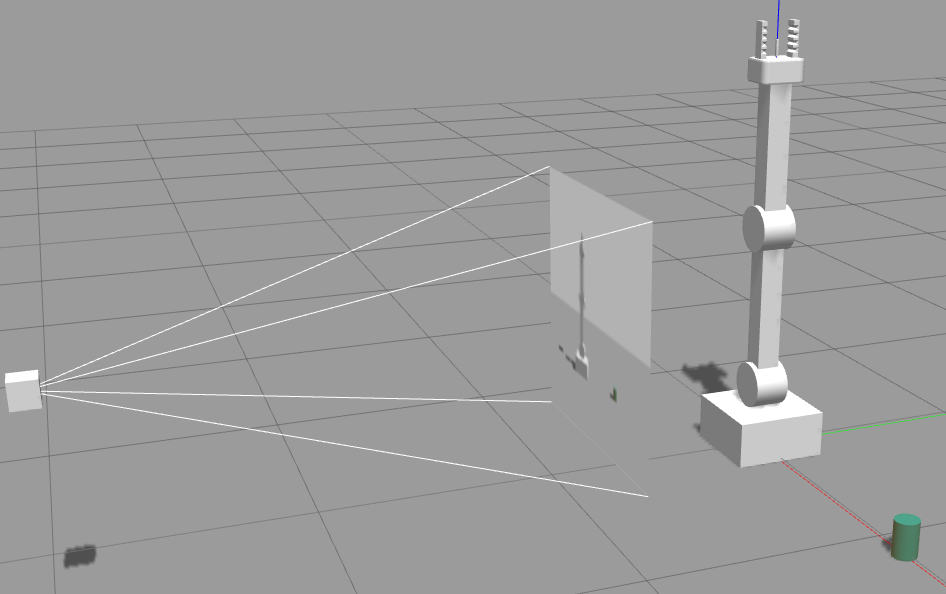
\includegraphics[width=0.6\textwidth]{img/deep_rl_arm}
    \end{center}
    \caption{Robot manipulator setup}
    \label{fig:deep_rl_arm}
\end{figure}
In task 1 of the project the entire arm of the manipulator is counted as valid collision target and an accuracy of 90\% successful touches over at least 100 attempts has to be achieved.

In task 2 only the base of the parallel jaw gripper attached to the endeffector is allowed to touch the can for a successful run and the accuracy has to exceed 80\% out of more than 100 iterations.

For all the experiments the base joint is locked, reducing the task to two degrees of freedom.

The agent could be set up to either operate on joint positions or joint velocities as control parameters.
The controlling agent has to choose between increasing or decreasing either of the two joints position/velocity. This yields 4 available actions the agent has to choose from at each time step, based on its policy and the provided input image state.

Through the use of reinforcement learning techniques the problem of training the agent can be solved by repeatedly letting it try to deduce actions based on the image and reward intended behaviour while penalizing erroneous actions.



%Have any part of the robot arm touch the object of interest, with at least a 90% accuracy for a minimum of 100 runs.
%The student should complete all tasks specified in the Classroom, with the end objective of the robot arm touching the object with at least a 90% accuracy for a minimum of 100 runs.
%Have only the gripper base of the robot arm touch the object, with at least a 80% accuracy for a minimum of 100 runs.
%The student should complete all tasks specified in the Classroom, with the end objective of the arm's gripper base touching the object with at least a 80% accuracy for a minimum of 100 runs.

\section{Reward Functions}  

The mechanisms used to reward the reinforcement learning agent are the following.
\begin{itemize}

    \item Whenever the agent sucessfully hits the can it receives REWARD\_WIN = 100 and the episode ends. In task 2 hitting the can with anything else but the gripper yields REWARD\_LOSS = -30.

    \item If the gripper ever hits the ground or the 100th simulation step is exceeded, the reward is REWARD\_LOSS = -30 and the episode is terminated.

    \item For each simulation step the average motion of the endeffector towards the goal ($avgGoalDelta$) is determined
    $$ avgGoalDelta \leftarrow \alpha * avgGoalDelta + (1 - \alpha) * distDelta $$
    where smoothing factor $\alpha = 0.2$ and $distDelta$ is the difference in endeffector-to-goal-distances of two consecutive steps.

    The resulting intermediate reward  that is issued every timestep is then comprised of a scaled motion based REWARD\_GOAL\_APPROACHING = 20 and a very small constant penalty of REWARD\_TIME\_PENALTY = -0.1.
    $$ reward = avgGoalDelta * 20 - 0.1 $$
    This yields positive rewards for average motion of the endeffector towards the goal.

\end{itemize}
%Explain the reward functions that you created.
%Brief explanation of each reward function and associated reward values. The writeup should also include what type of joint control was implemented.

\section{Hyperparameters}  
%Specify the hyperparameters that you selected for each objective, and explain the reasoning behind the selection.
%Student should explain the choice of hyperparameters for both objectives.
The agents created for task 1 and task 2 operated on changing the joint positions with each sampled action. 

Table~\ref{tab:hyperparameters} hyperparameters gives provides a summary for the hyperparameters described in this section that are used to train were agent for both tasks:
\begin{figure}[thpb]
    \centering
    \begin{tabular}{|c|c|}\hline
        INPUT\_WIDTH  & 64  \\ 
        INPUT\_HEIGHT & 64  \\ 
        OPTIMIZER & RMSprop  \\ 
        LEARNING\_RATE & 0.05 \\ 
        REPLAY\_MEMORY & 10000  \\ 
        BATCH\_SIZE & 128  \\ 
        USE\_LSTM & false  \\ 
        LSTM\_SIZE & \# \\ \hline

        EPS\_START  & 0.9f \\
        EPS\_END  & 0.01f \\
        EPS\_DECAY  & 200 \\
        \hline
    \end{tabular}
    \caption{Hyperparameters}
    \label{tab:hyperparameters}
\end{figure}

\subsection*{INPUT\_WIDTH x INPUT\_HEIGHT} 
The camera image that acts as state input for the agent is downsized to a 64x64pixels image to reduce state and model complexity while still providing enough information and resolution to sufficiently identify the required elements in the scenery.

\subsection*{OPTIMIZER}
During tuning of the hyperparameters Adam as well as RMSprop were evaluated and appeared to yield essentially the same results. RMSprop was chosen for the final training of both task 1 and task 2.

\subsection*{LEARNING\_RATE} 
The step size the optimizer takes after evaluating the gradient descent vector is scaled by the LEARNING\_RATE. It gives control over the tradeoff between speed of convergence of the learning algorithm convergence stability. After launching several training cycles with learning rates of 0.2, 0.1, 0.05 or 0.01 it became clear that eventhough higher learning rates also occasionally were able to learn good behaviour, the final rate of 0.05 repeatedly yielded successful agents.

\subsection*{REPLAY\_MEMORY} 
The size of the experience pool the algorithm retains to sample from for each policy update step is determined by the REPLAY\_MEMORY parameter. Setting this size to 10000, as done to achieve the results for task 1 and task 2, means the agent stores its past 10000 experiences in a first in first out manner and randomly recalls a batch of BATCH\_SIZE form this pool to improve its policy.

\subsection*{USE\_LSTM \& LSTM\_SIZE} 
After training several agents using an LSTM layer of 16, 64 and 128 nodes it was observed that many of these agents quickly ran into overfitting to some suboptimal policy, while some achieved relatively good accuracy. Omitting the use of the LSTM layer produced much more stable learning results and therefore USE\_LSTM was set to false for the final agents. I hypothesize that having an LSTM layer to retain temporal information might be beneficial for the task at hand but this layer seems to be comparably difficult to train appropriately.

\subsection*{EPS} 
The EPS parameters, controlling the rate of exploration vs exploitation were changed to start at EPS\_START 0.9 and exponentially decay over EPS\_DECAY 200 steps to EPS\_END 0.01. This means the agent starts out with 90\% of actions being randomly chosen but once the policy starts to converge the remaining small amount of just 1\% exploration allow the controller to exploit the learned policy.


\section{Results}  

The video available at \href{https://youtu.be/n06wDGm7ll4}{https://youtu.be/n06wDGm7ll4} show the training of the agent for task 1 where it's allowed to touch the can with any part of the arm to get full reward.
The final accuracy of the agent reaches 92.06\% as shown in Fig~\ref{fig:task1_final}.

\begin{figure}[thpb]
    \centering
    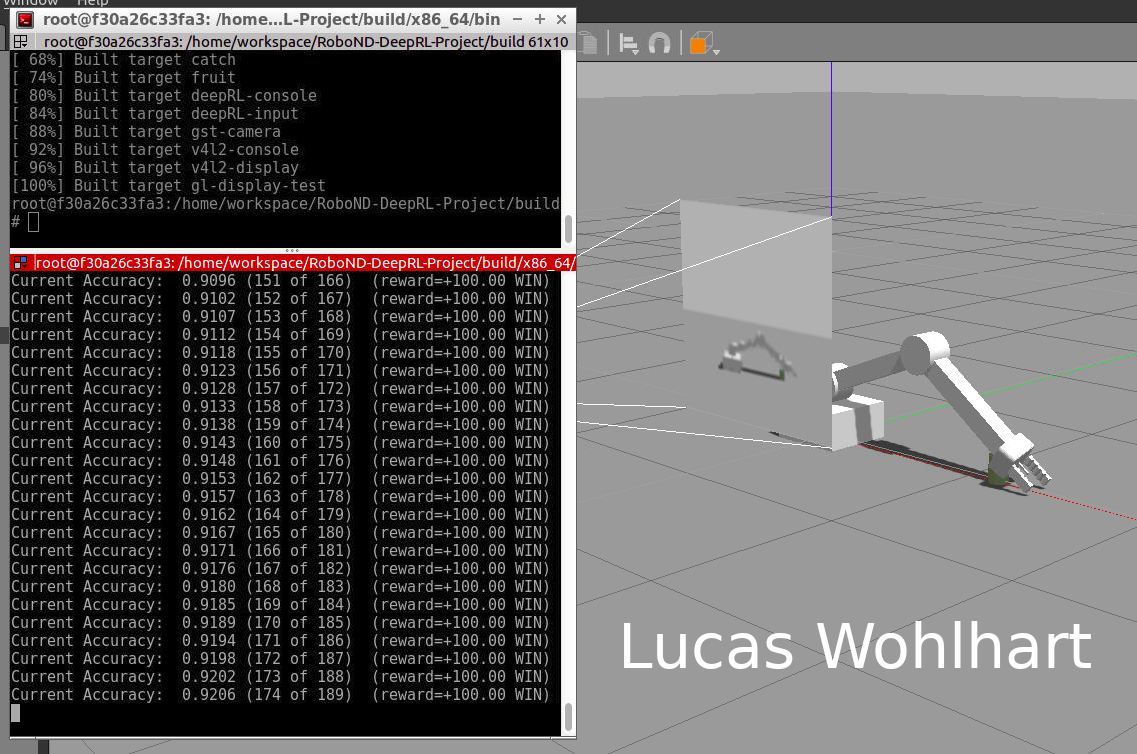
\includegraphics[width=0.85\linewidth]{img/task1_final.png}
    \caption{Task 1 final accuracy}
    \label{fig:task1_final}
\end{figure}

The video \href{https://youtu.be/frCadMNOyA0}{https://youtu.be/frCadMNOyA0} shows some parts of the training of the agent for task 2. At first the agent struggles to find the most rewarding goal at all. Once it reaches this goal it is capable of optimizing for this behaviours. Every now and then the already good policy seems to deteriorate a bit for a small period of time. It starts to consecutively miss the target for a short time span of 3 or 4 episodes eventhough the residual exploration probability is down to approximately 1\%.

The final accuracy of the agent reaches 82.97\% as shown in Fig~\ref{fig:task2_final}.


\begin{figure}[thpb]
    \centering
    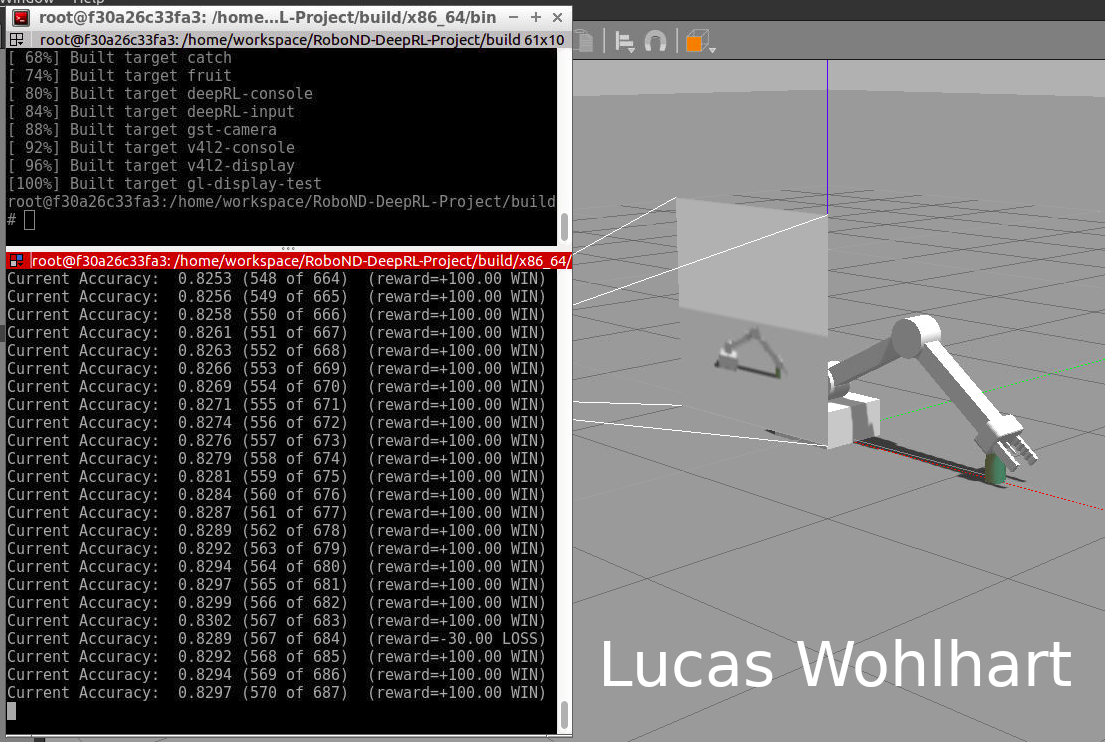
\includegraphics[width=0.85\linewidth]{img/task2_final.png}
    \caption{Task 2 final accuracy}
    \label{fig:task2_final}
\end{figure}

%Explain the results obtained for both objectives. Include discussion on the DQN agent's performance for both objectives. Include watermarked images, or videos of your results.
%Student should describe and briefly explain the results they achieved for both objectives. The discussion should also include their comments on the DQN agent's performance and if there were any shortcomings. Student should include either watermarked images of their results, or attach a video that displays the results and the arm in action.

\section{Future Work}  

As always, hyperparameter search is a tedious process but once a reasonable configuration is found the creation of intelligent agents by simply reinforcing intended behaviour is a truely amazing approach.

Randomizing the target object position as well as the initial pose of the manipulator would be a very interesting next extension to this experiment. Also unlocking the base-joint of the arm or even mounting the manipulator on a mobile base (such as a differential drive robot) to ultimately train a mobile manipulator with reinforcement learning could yield very promising results for flexbile industry scenarios.

Overall the agent was able to perform both required tasks. However, it would have been wise to first just train the agent and evaluate this model, regarding the task requirements, without residual action noise. This would allow the use of much more exploration noise during training to truely cover the entire state space and achieve more than just one or two successful motion patterns.


%Briefly discuss how you can improve your current results.
%Student should discuss on what approaches they could take to improve their results.


% \bibliography{bib}
%\bibliographystyle{ieeetr}

\end{document}